\section{Frontend}

The evaluation of the Elephant browser and the NetInfService applications tries to answer the following core questions:

\begin{enumerate}
\item How much uplink bandwidth is saved?
\item How much content is reused?
\item How much of linked resources are dynamically generated?
\item How fast is the browser?
\end{enumerate}

\subsection{Test Setup}

The first test consists of a set of web pages and four Android phones. Each phone will automatically retrieve the set of pages in a random order.
Using the logging functionality of the 
applications, information about how (Internet, Bluetooth, NRS or Database) 
resources are retrieved is gathered. Information about how many bytes each resource consists of 
and how long it takes to retrieve is also acquired. Full put is 
enabled on all four phones, because the answer to question one 
does not depend on which method of transfer is used. 
The results are meant to give an idea of the answer to 
questions one and two.

The web page sets are of sizes 15, 20, 25 and 30. 
They are derived from the service Alexa \cite{alexa},
which is renowned for its web metrics. 
This service keeps track of the most visited web sites by country, 
and the top sites were used to create the sets.

The test also uses a 
Name Resolution Service that is reset between retrieving each set of web pages.

The second test setup consisted of two runs: First, 
retrieving all web pages in the set of 15 web pages using one blank
phone. Second, the same phone retrieves the same set of web pages again. This time, the phone should already have the web pages in its database.
The results are meant to give an idea of the answer to question three. 
The test is repeated two times, with the Name Resolution Service 
reset in between. 

A third test uses four phones, each retrieves the 15 web pages set. 
This test is repeated three times once with full put enabled on all phones, once with full put enabled 
on two phones and finally with full put disabled on all phones. 
This is done to test the Bluetooth functionality. 
The goal of this test is to simulate the scenarios where there is no, limited, or full peer-to-peer interaction, respectively.

\subsection{Hardware}

The tests are run on three Samsung Galaxy Nexus phones and one 
HTC One X phone using Android OS 4.1.1 Jellybean

The Name Resolution Service was run on an 
Intel Core 2 Quad CPU Q9400 @ 2.66GHz × 4 with 4 gigabytes 
of volatile memory using Ubuntu 12.04 LTS.

\subsection{Limitations}

The Name Resolution Service supports two types of databases for storing published NDOs. The first uses Erlang 
lists stored in volatile memory, the other uses a Riak database. 
The tests use the list database as it was the database used during the development of the browser application.

This means that the test is limited by the amount of free 
volatile memory of the system. A preliminary test using a set of 50 web 
pages caused the system to run out of memory, resulting in a crash. 
Because of this, no set contains more than 30 web pages.

\subsection{Results}

% Plot of usage

% Table comparing time of access to each resource

% Table (or plot) of re-usage after period

The results of test one can be seen in Figure \ref{fig:frontendtest1}. Each bar represents a 
specific set size and the colors show how much of the data was transferred with each technology.

Table \ref{tbl:times} shows the total time spent and the time spent transferring the files while retrieving 
the 15 web page set.

The results of test two can be seen in Figure \ref{fig:frontendtest2}. The two leftmost bars represent 
the first run of the test and the two rightmost the second.

The results of the third test can be seen in Figure \ref{fig:frontendtest3}


\begin{figure}[H]
	\centering
		\includegraphics[width=0.62\textwidth, angle=-90]{./img/overall.pdf}
    	\caption{Percentage of data transferred over the different transport methods during test one}
	\label{fig:frontendtest1}
\end{figure}


\begin{table}[H]
		\centering
       \begin{tabular}{| c | c | c | c |}
               \hline
               Phone \# & Total time (s) & Time downloading (s) & Time downloading (\%)\\
               \hline
               1 & 251 & 17 & \textbf{6}\\
               \hline
               2 & 303 & 15 & \textbf{4}\\
               \hline
               3 & 241 & 20 & \textbf{8}\\
               \hline
               4 & 254 & 18 & \textbf{7}\\
               \hline
       \end{tabular}
       \caption{Total time and time spent downloading for the set of 15 web pages used during test one}
       \label{tbl:times}
\end{table}


\begin{figure}[H]
	\centering
		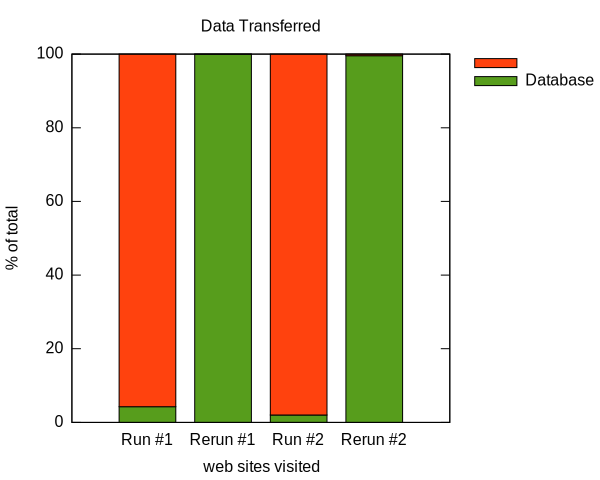
\includegraphics[width=0.62\textwidth, angle=-90]{./img/rerun.pdf}
    	\caption{Percentage of data retrieved from the local database during test two}
	\label{fig:frontendtest2}
\end{figure}

\begin{figure}[H]
	\centering
		\includegraphics[width=0.62\textwidth, angle=-90]{./img/bt.pdf}
    	\caption{Percentage of data transferred over the different transport methods during test three}
	\label{fig:frontendtest3}
\end{figure}

\subsection{Discussion}

Figure \ref{fig:frontendtest1} shows that approximately 30\% of the data 
can be retrieved without accessing the Internet. Precaching of popular web pages is expected to improve this result.

It was observed that if one phone had a jump start on another phone when retrieving a certain web page, 
the second phone shortly caught up with the first phone. The two phones would then try to retrieve the same resource 
at the same time. Since this resource will not be in the NRS, both phones will retrieve it from the Internet.

In Figure \ref{fig:frontendtest1} it can be seen that a few percent of the resources are retrieved from the 
database. The reason behind this is that some resources are reused multiple times throughout the web pages. 
Since resources are cached in the database the first time they are retrieved, additional requests can use the cached version.

Figure \ref{fig:frontendtest2} demonstrates that when accessing a web page a second time, a small part still has to be 
retrieved using the Internet. An example of when this can happen is when a web page links to a resource using JavaScript 
to add a timestamp to the resource's URL. Because of the dynamic nature of this content, it will not be found when searched for. Therefore, there will be a small amount of resources that always will be retrieved from the Internet.

In Figure \ref{fig:frontendtest3} the amount of data retrieved without using the Internet is similar 
whether or not full put was used. This is as expected because the data that is not made available through full put should 
be available through Bluetooth. 

An unexpected behavior observed during testing is that the application spends most of the time searching. More specifically, the NRS does not respond in a timely manner to requests that result in no match. Unfortunately, the time spent searching is not logged. As can be seen in Figure \ref{tbl:times} the time downloading is a small fraction of the total time spent. It is strongly suspected that most of the total retrieval time is spent waiting for search results.

A second unexpected behavior observed is that the NetInfService randomly pauses until it regains focus. When this happens all NetInf functionality becomes unavailable, which causes all resources to be retrieved from the Internet. It is suspected that this is caused by how the Android OS handles background applications.

